%%%%%%%%%%%%%%%%%%%%%%%%%%%%%%%%%%%%%%%%%%%%%%%%%%%%%%%%%%%%%%%%%%%%%%%
% Created on Mon Dec 6, 2023
% @author: Giselle Labrador Badia (@gisslab)


% Description:
%
% This shows reports on the DID exposure analysis.


%%%%%%%%%%%%%%%%%%%%%%%%%%%%%%%%%%%%%%%%%%%%%%%%%%%%%%%%%%%%%%%%%%%%%%%




\documentclass[11pt,a4paper]{article}


\usepackage[utf8]{inputenc}
\usepackage[spanish,english]{babel}
\usepackage{apacite}
\usepackage[round]{natbib}
\usepackage{hyperref}
\bibliographystyle{apacite}


\usepackage[margin = 1in, top=2.0cm,bottom=1.5cm]{geometry}% Margins
\setlength{\parindent}{2em}
\setlength{\parskip}{0.3em}
\usepackage{setspace} % Setting the spacing between lines
\usepackage{hyperref} % To create hyperlinks within the document
\spacing{1.15}

%images
\usepackage{graphicx}
% \usepackage{subcaption}
\usepackage{caption}
% subcaption was interfering with the figure count, fix below
\usepackage{subcaption, xparse}

% to read mid-rule
\usepackage{booktabs}

\usepackage[capposition=top]{floatrow}
\captionsetup[sub]{font=footnotesize,labelfont={bf,sf}}

\begin{document}

\title{Effects of QE on O.B. Auctions \\ Dynamic DiD Exposure Analysis}

\maketitle

\section{FED purchases and investors}

The following figures show the daily time series of amounts and prices of FED purchases of MBAs for Fannie Mae and Freddie Mac
 products and 30-year maturity in the early COVID period. We plot by month the total amount by coupon and the mean price. 
 %If it only shows a dot is because there is only one month of data for that coupon. The period is January 2020 to April 2021. 
 The prices and quantities are aggregated monthly by trade date. 


\begin{figure}[h]
    \centering
    \begin{subfigure}[b]{0.49\textwidth}
      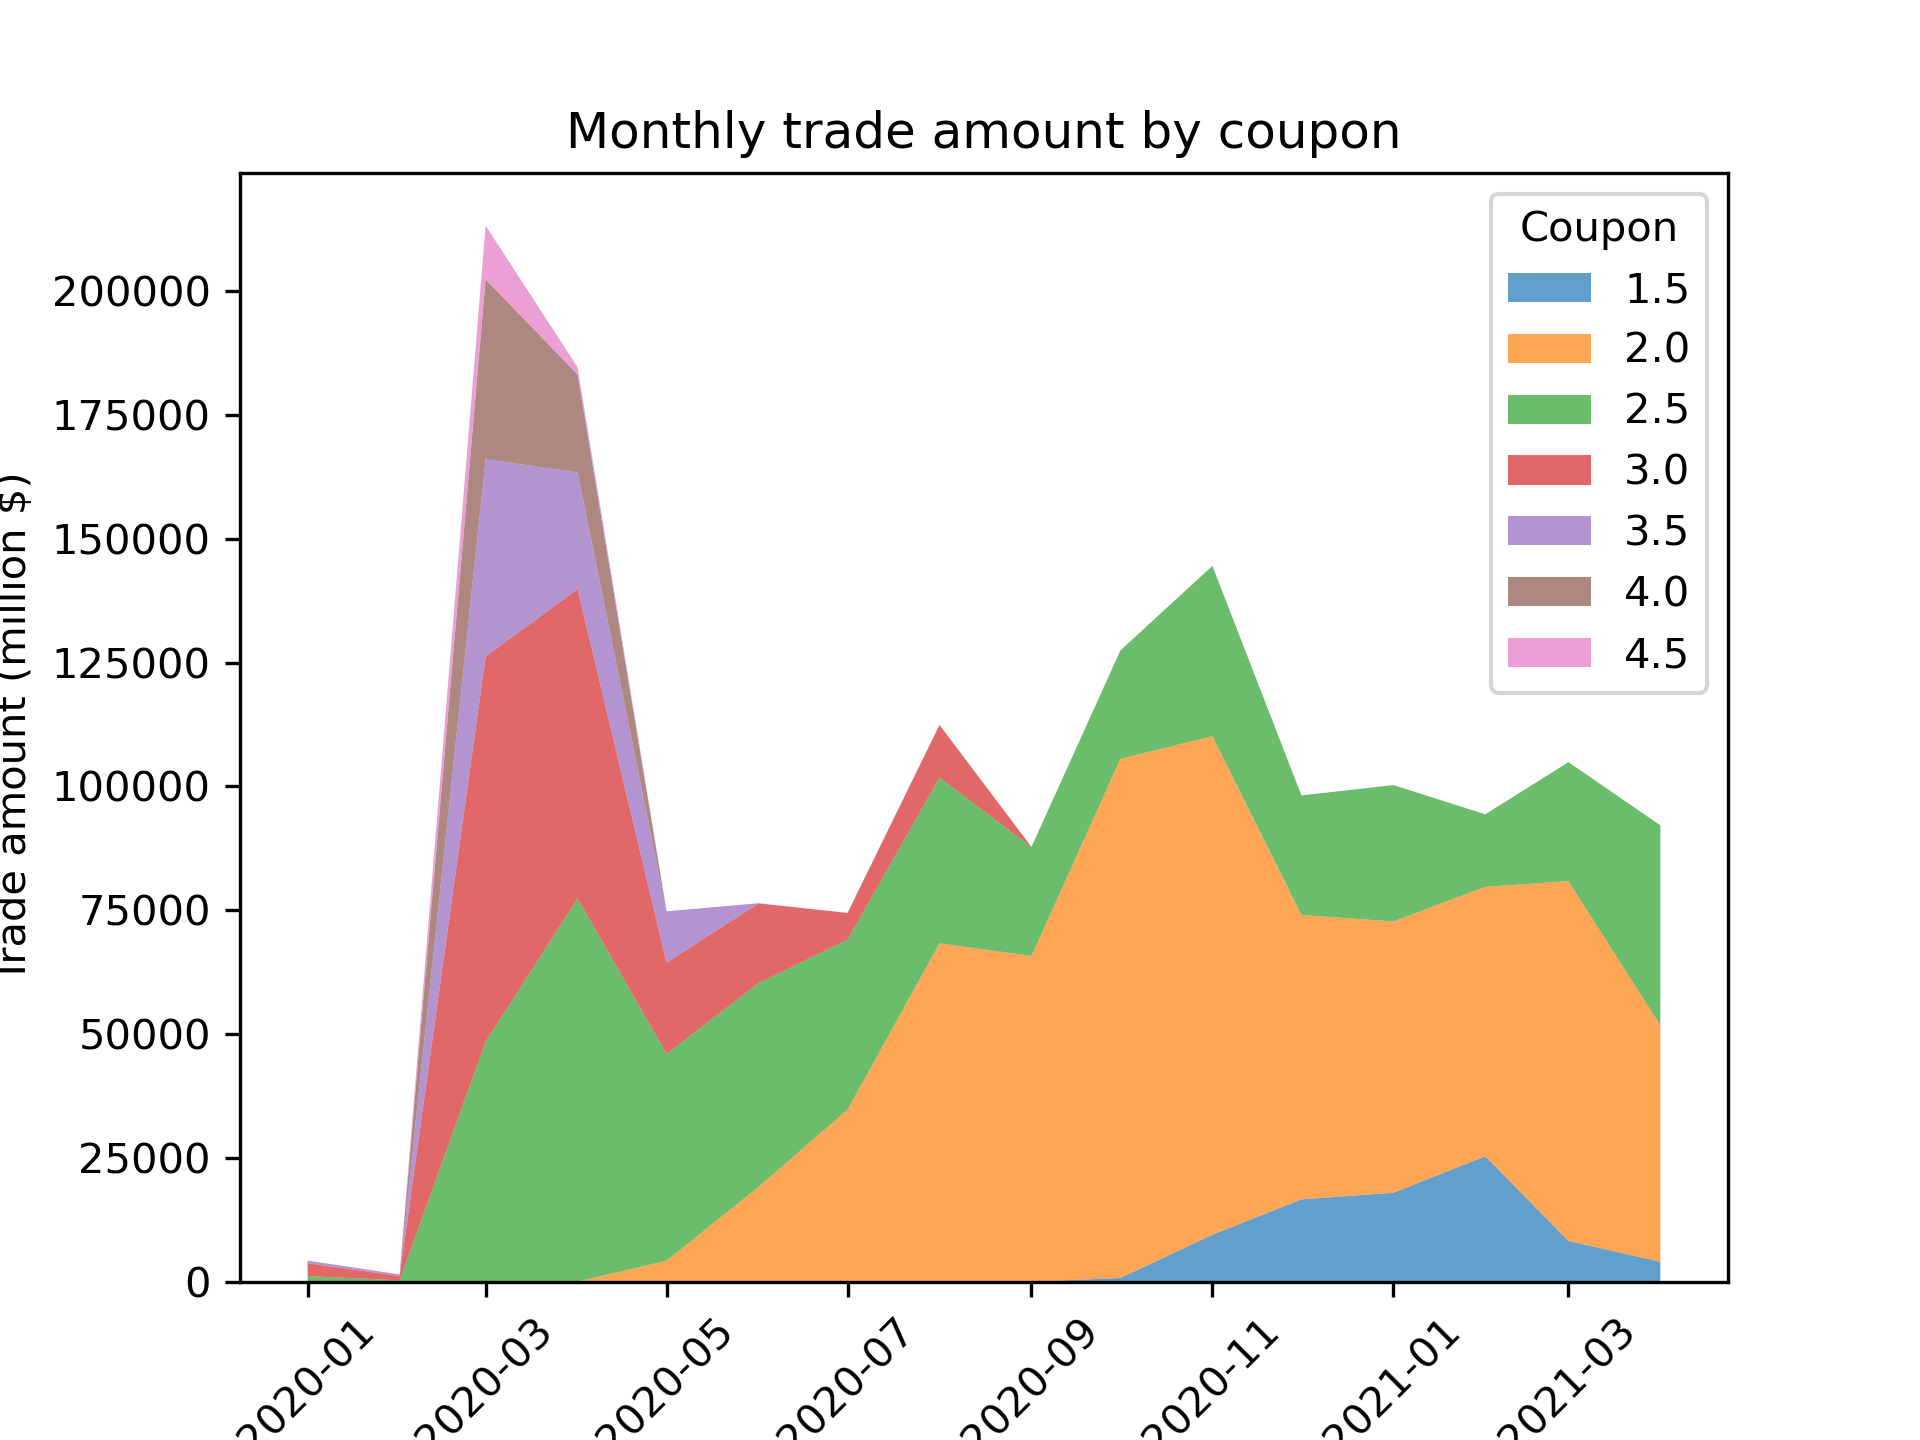
\includegraphics[width=0.998\textwidth]{../results/figures/fed_monthly_trade_amount_by_coupon.png}
      \caption{ Quantity by trade date}
     \end{subfigure}
     \begin{subfigure}[b]{0.49\textwidth}
      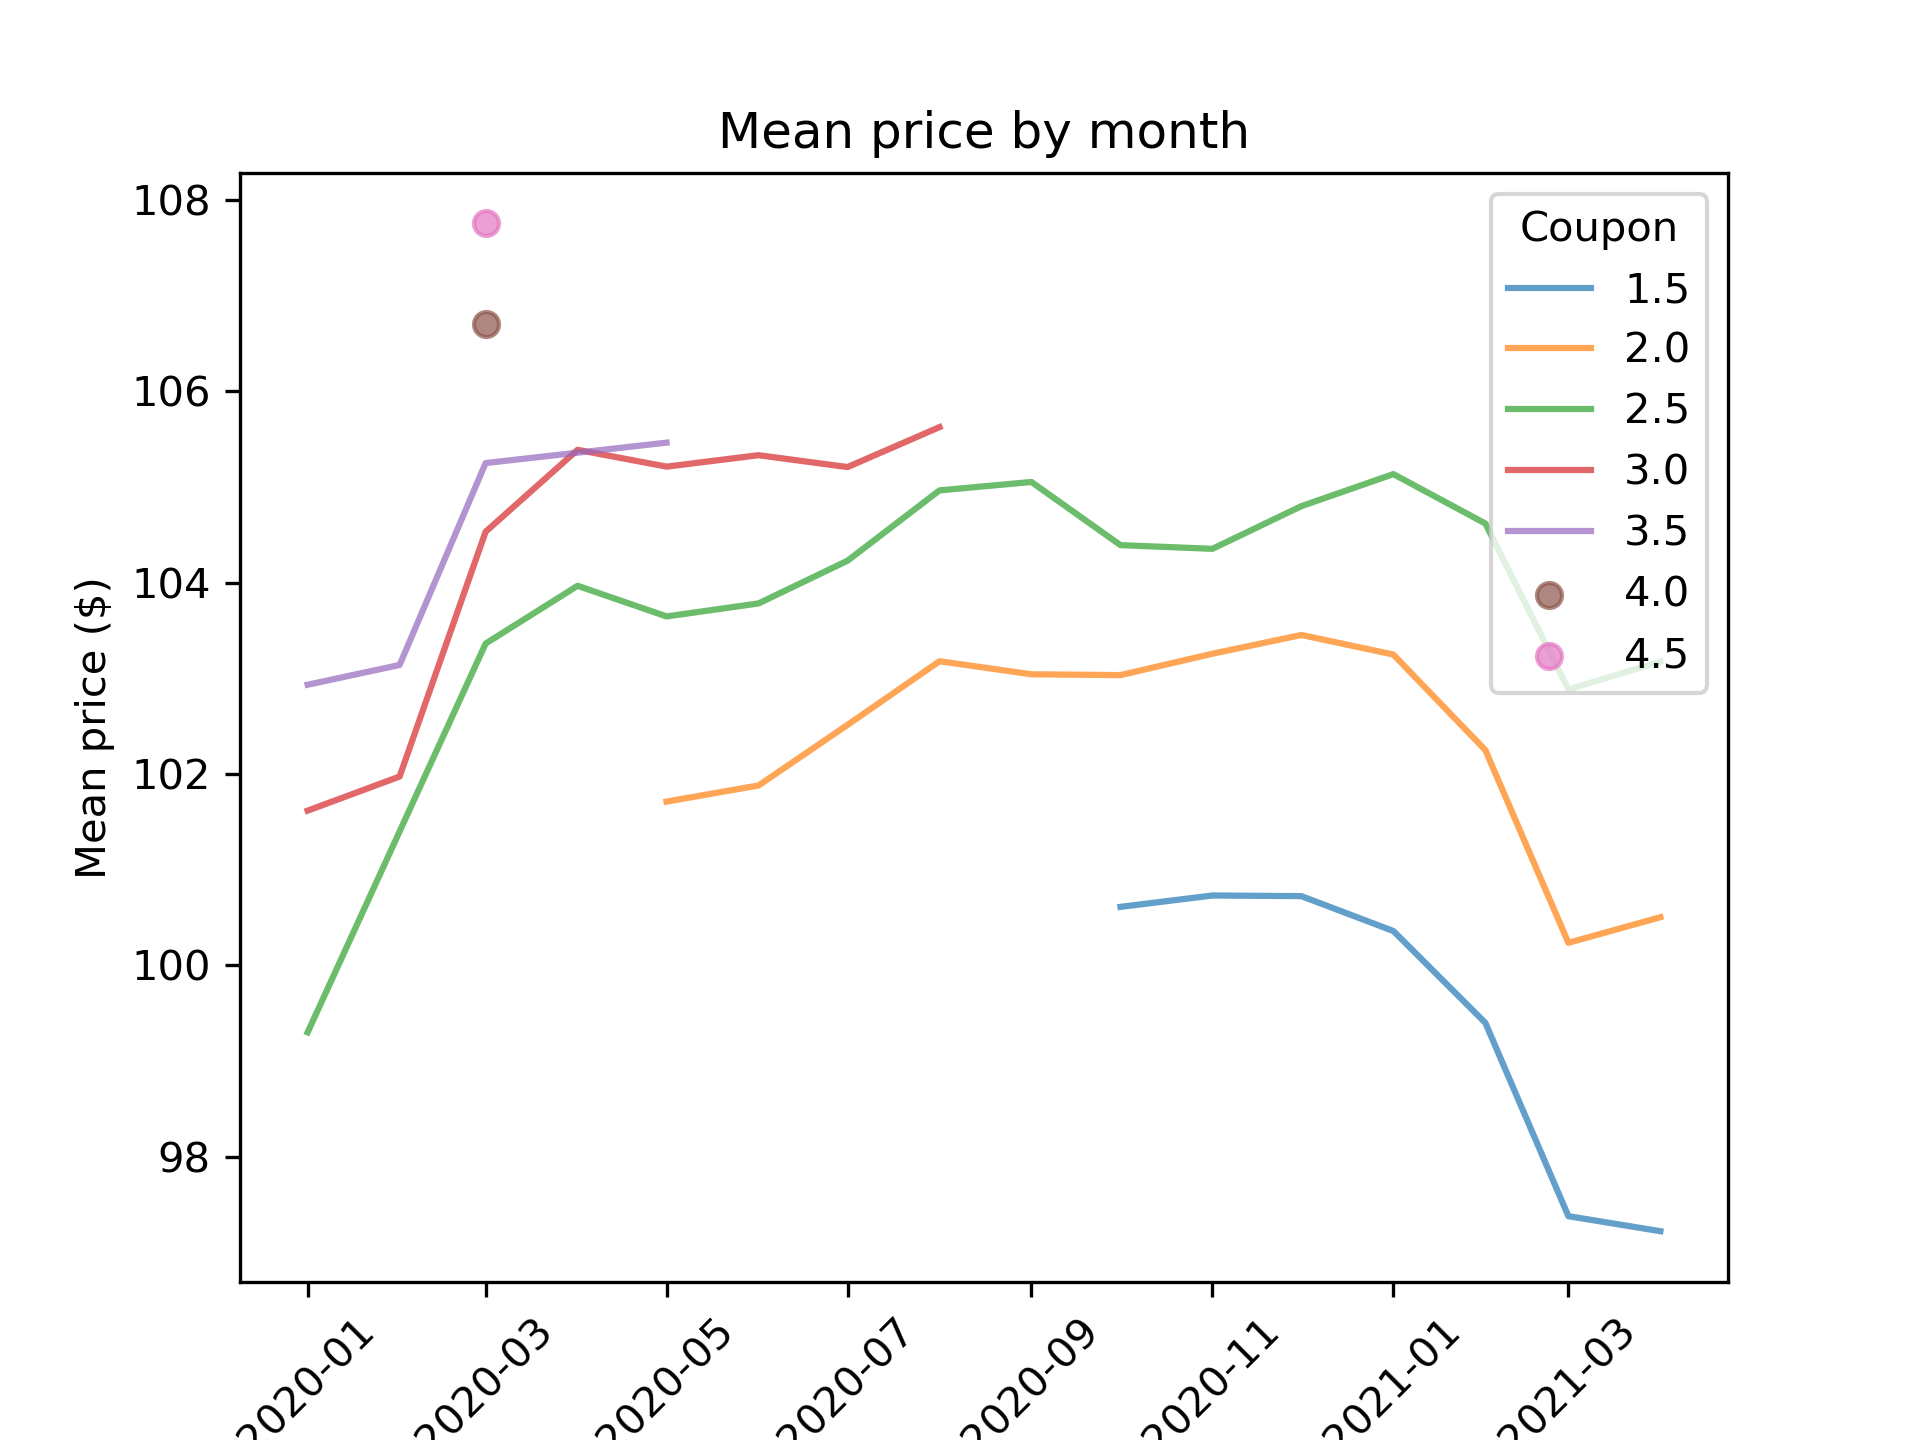
\includegraphics[width=0.998\textwidth]{../results/figures/fed_monthly_price_mean_by_coupon.png}
      \caption{ Price by trade date}
     \end{subfigure}
     \caption{FED purchases of Fannie Mae and Freddie Mac MBS securities  in the early COVID period} 
     \begin{minipage}{\textwidth}
      \footnotesize{\textit{Notes:} The figure shows the monthly time series of trade amounts and prices of FED purchases of Fanny Mae and Fredy Mac products and 30-year maturity. Colors represent different coupons. } 
        \end{minipage}
\end{figure}

\pagebreak

Below, we show the amount of MBS purchased by the FED to each investor.
\begin{table}[h]
    \centering
    \begin{tabular}{lr}
\toprule
                         Counterparty &  Amount (millions \$) \\
\midrule
             Morgan Stanley \& Co. LLC &        304942.000000 \\
    Credit Suisse AG, New York Branch &        250823.000000 \\
        Citigroup Global Markets Inc. &        147080.000000 \\
              Goldman Sachs \& Co. LLC &        135429.000000 \\
                BofA Securities, Inc. &        120978.000000 \\
                    J.P. Morgan Chase &        107276.000064 \\
               Wells Fargo Securities &         85703.000000 \\
                Barclays Capital Inc. &         75758.000000 \\
Nomura Securities International, Inc. &         72998.999872 \\
   Daiwa Capital Markets America Inc. &         46478.000000 \\
                          BNP-Paribas &         17412.000000 \\
            Mizuho Securities USA LLC &          9715.000000 \\
                        Jefferies LLC &          6345.000000 \\
\bottomrule
\end{tabular}

    \caption{Sold amount in period Jul 2019 to April 2021}\label{tab:descriptive}
    % \begin{minipage}{\textwidth}
    %     \footnotesize{\textit{Notes:}  } 
    %     \end{minipage}
\end{table}

There are 931 from  14873 observations in this period that have a missing counterparty (investor).

\pagebreak
\begin{figure}[h]
    \centering
    \begin{subfigure}[b]{0.7\textwidth}
        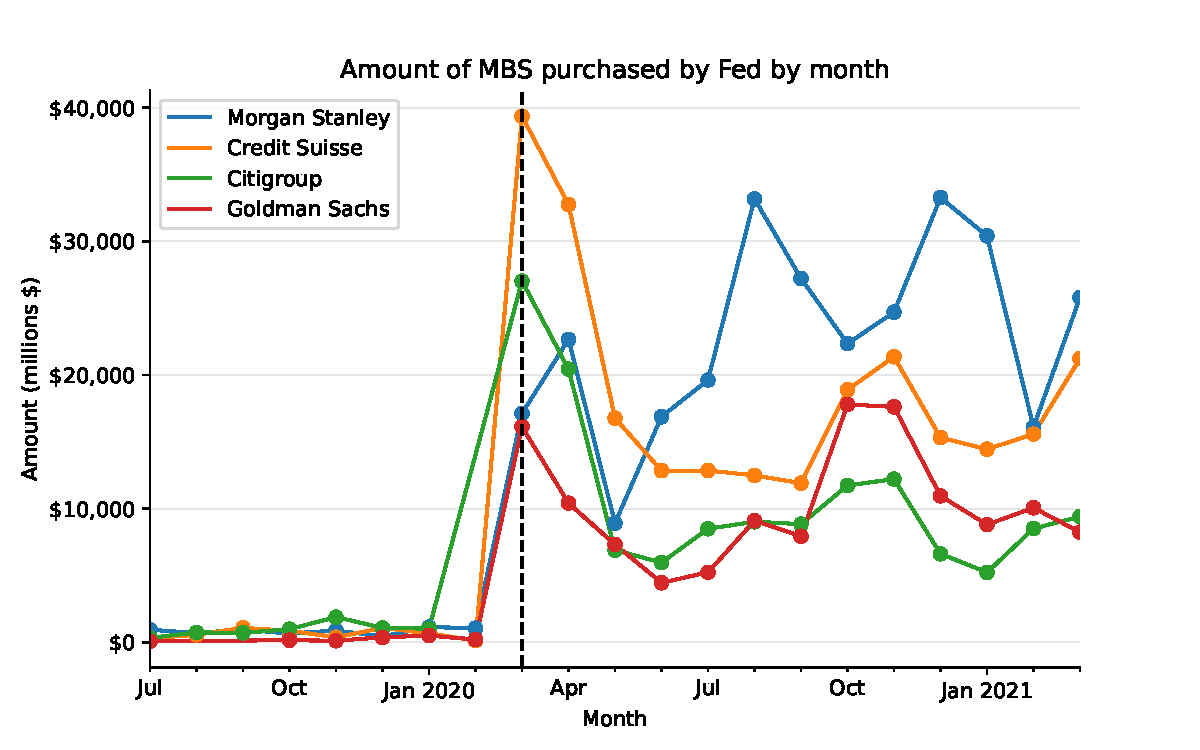
\includegraphics[width=0.98\textwidth]{../results/figures/fed_mbs_amount_by_month_example_larg4.pdf}
        \caption{Largest 4 investors that sold loans to the FED.}\label{fig:larg4}
       \end{subfigure}
       \begin{subfigure}[b]{0.7\textwidth}
        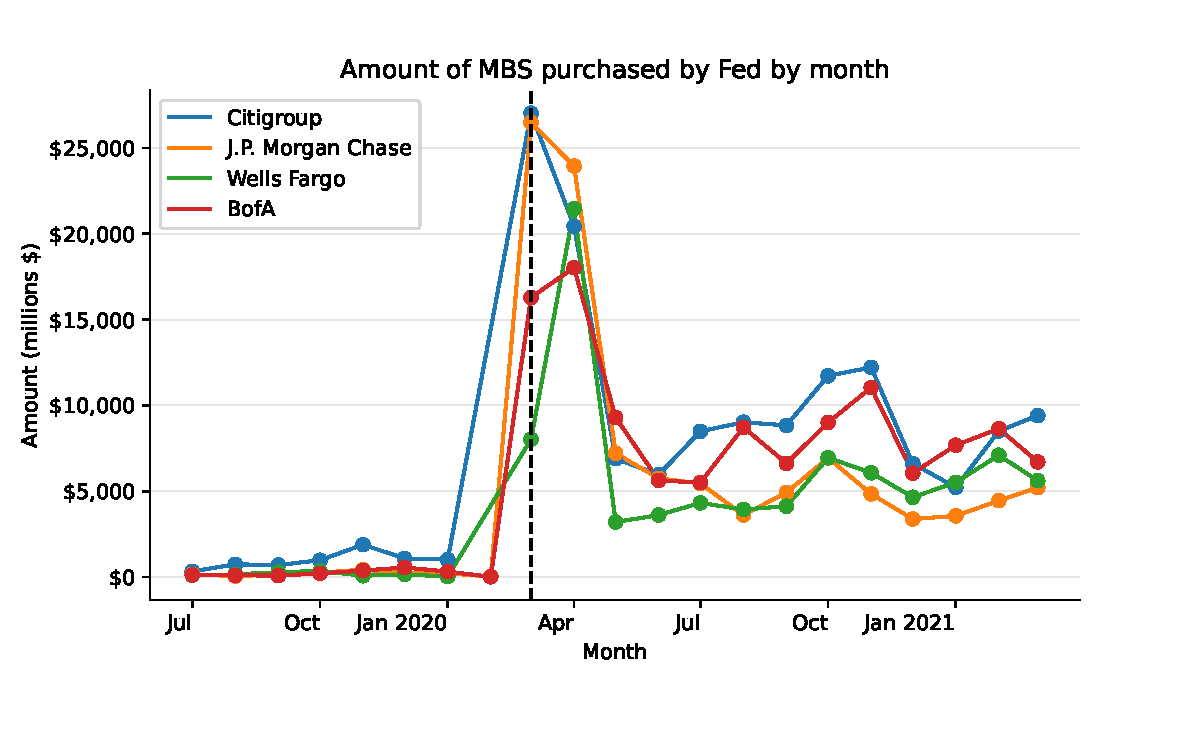
\includegraphics[width=0.999\textwidth]{../results/figures/fed_mbs_amount_by_month_example_retail.pdf}
        \caption{ Commercial banks } 
       \end{subfigure}
       \caption{FED MBS purchases by month.}\label{fig:fed_mbs_amount_by_month}
     \begin{minipage}{\textwidth}
        \footnotesize{\textit{Notes:} The figure shows a time series of FED auction outcomes. The vertical line is March 1.  } 
        \end{minipage}
  \end{figure}


%   \begin{figure}[h]
%     \centering
%        \begin{subfigure}[b]{0.6\textwidth}
%         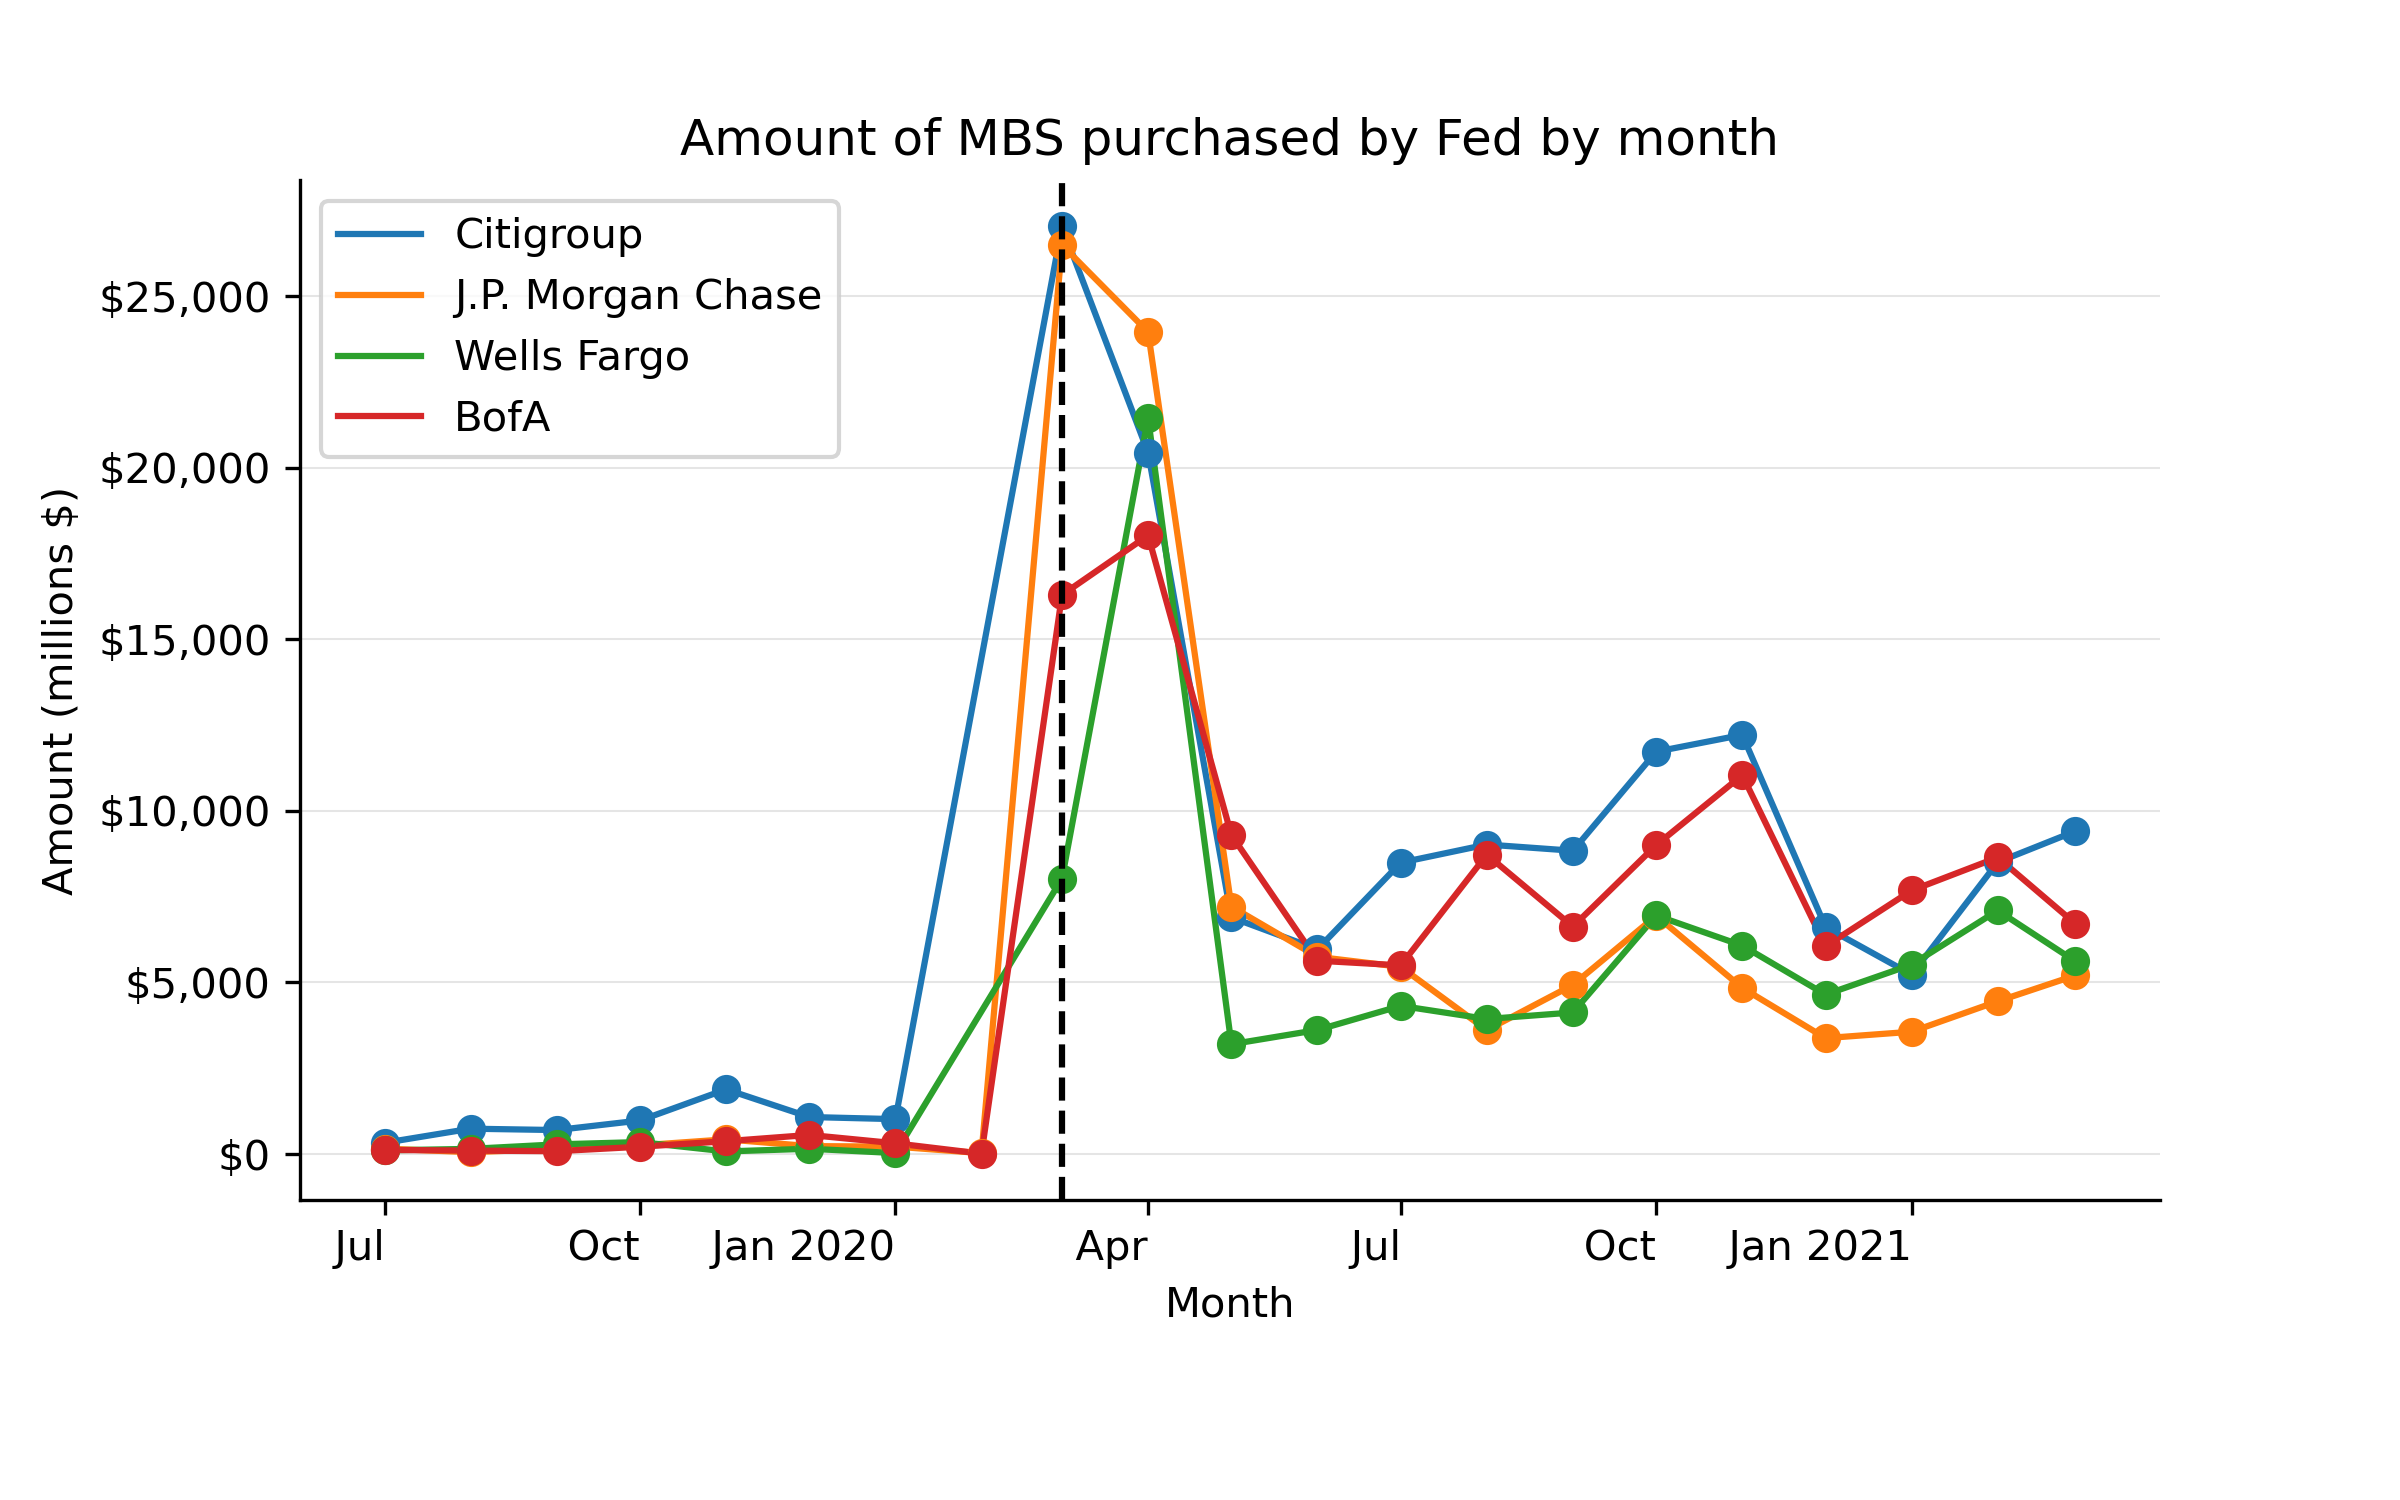
\includegraphics[width=0.999\textwidth]{../results/figures/fed_mbs_amount_by_month_example_retail.png}
%         \caption{ Bid difference between Freddie and Fannie.}
%        \end{subfigure}
%        \caption{OB auction  GSE response for coupon 2.5 } 
%      \begin{minipage}{\textwidth}
%         \footnotesize{\textit{Notes:} The figure shows a time series of FED auction outcomes. The vertical line is March 1.  } 
%         \end{minipage}
%   \end{figure}

\pagebreak

\subsection{FED purchases and O.B. Auctions}

\begin{figure}[h]
  \centering
  \begin{subfigure}[b]{0.7\textwidth}
    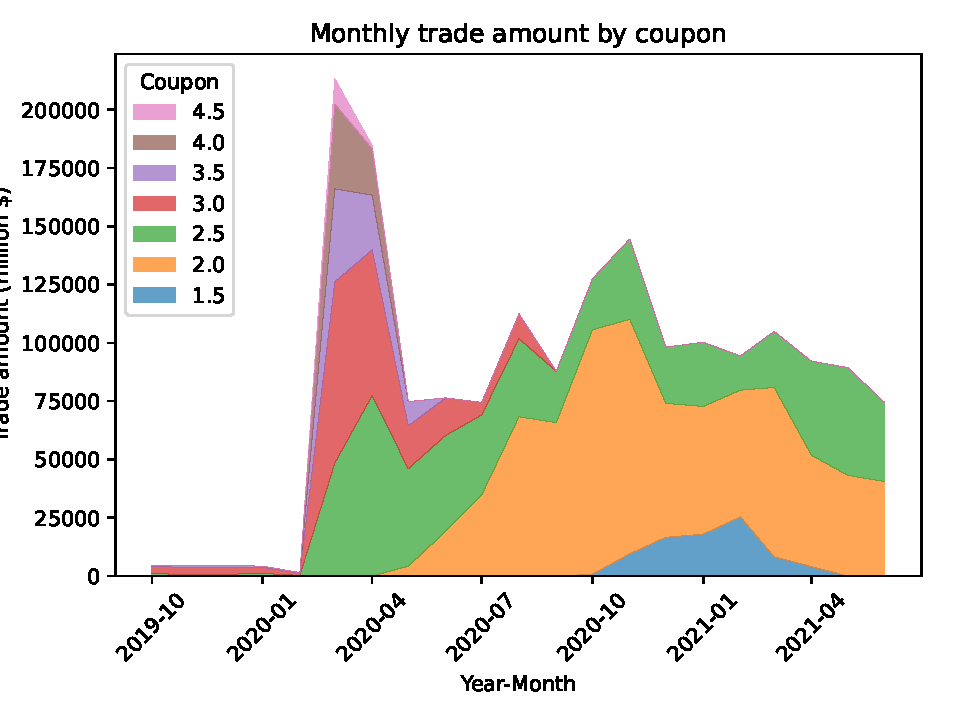
\includegraphics[width=0.998\textwidth]{../results/figures/fed_monthly_trade_amount_by_coupon.pdf}
    \caption{FED purchases}
   \end{subfigure}
   \begin{subfigure}[b]{0.7\textwidth}
    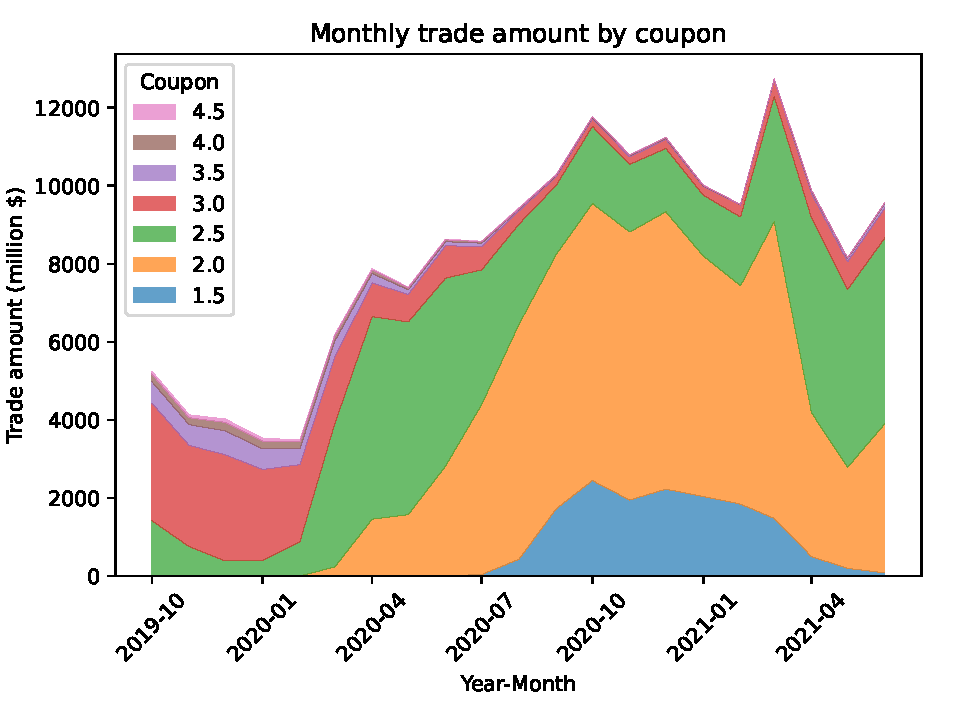
\includegraphics[width=0.998\textwidth]{../results/figures/ob_monthly_trade_amount_by_coupon_all_area.pdf}
    \caption{OB total amounts}
   \end{subfigure}
   \caption{FED purchases of Fannie Mae and Freddie Mac MBS securities comparison.} 
   \begin{minipage}{\textwidth}
    \footnotesize{\textit{Notes:} The figure shows the monthly time series of trade amounts and prices of FED purchases of Fanny Mae and Fredy Mac products and 30-year maturity by coupon or noterates. } 
      \end{minipage}
\end{figure}


% ob_monthly_trade_amount_by_noterate_all_area_legend_colors.pdf

\begin{figure}[h]
  \centering
  % \begin{subfigure}[b]{0.75\textwidth}
  %   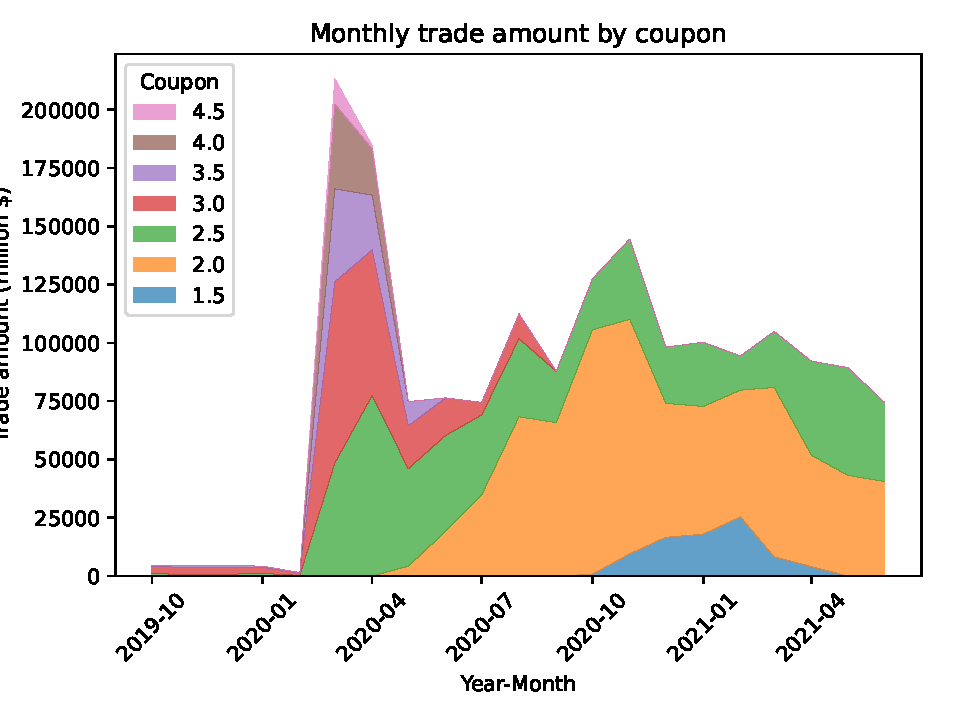
\includegraphics[width=0.998\textwidth]{../results/figures/fed_monthly_trade_amount_by_coupon.pdf}
  %   \caption{FED purchases}
  %  \end{subfigure}
   \begin{subfigure}[b]{0.75\textwidth}
    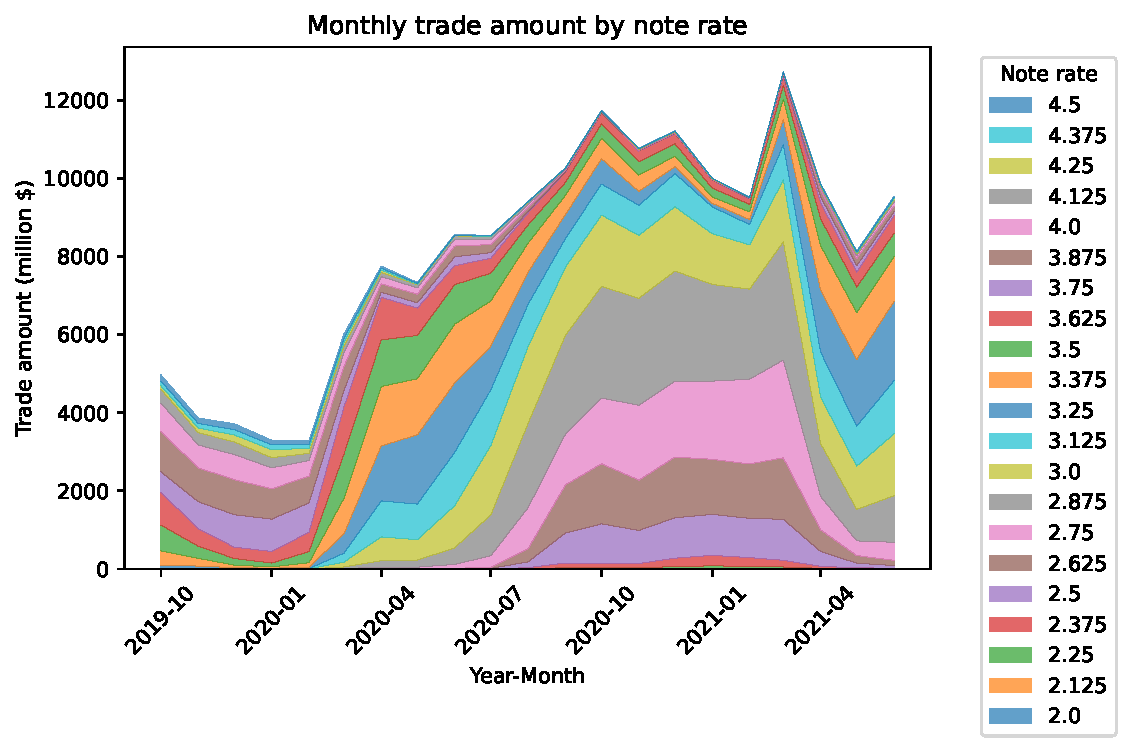
\includegraphics[width=0.998\textwidth]{../results/figures/ob_monthly_trade_amount_by_noterate_all_area_legend_colors.pdf}
    \caption{OB total amounts}
   \end{subfigure}
   \caption{OB auction note rate amounts} 
   \begin{minipage}{\textwidth}
    \footnotesize{\textit{Notes:} The figure shows the monthly time series of trade amounts and prices of FED purchases of Fanny Mae and Fredy Mac products and 30-year maturity by coupon or noterates. } 
      \end{minipage}
\end{figure}



\pagebreak
\section{Dynamic DiD Exposure Analysis}

The dynamic DiD analysis is based on the following equation:
$$y_{ijtc} = \alpha + \sum_\tau \beta_\tau \times 1({\tau}=t)  \times QE_{ic} + \nu_{t,c} + \nu_{t,i} +\psi_{j} + \epsilon_{ijtc}$$
where $y_{ijtc}$ is rate of winner bid or loan amount for loans sold to investor $i$ from seller $j$ in month $t$ for coupon segment $c$. The variable $QE_{i}$ is either the exposure dummy or the exposure level. The exposure level is defined as the amount of MBS purchased by the FED in March 2020. When a dummy is used, the variable takes the value of 1 if the investor has exposure and 0 otherwise. 

The investors that we could identify as having exposure are J.P. Morgan Chase, Wells Fargo, and Citibank. The results are shown below.  The clearer effect is on the winning bid, there is an increase in the average winning bid after March 2020 for the exposed investors. Robustness checks on the fixed effects did not change the results.

There is plenty of run for improvements here (more controls, improve crosswalks, use differences, logs, other outcomes like probability of wining, bid, use spread instead of winner bid, etc).
\begin{figure}[h]
    \centering
    \begin{subfigure}[b]{0.49\textwidth}
        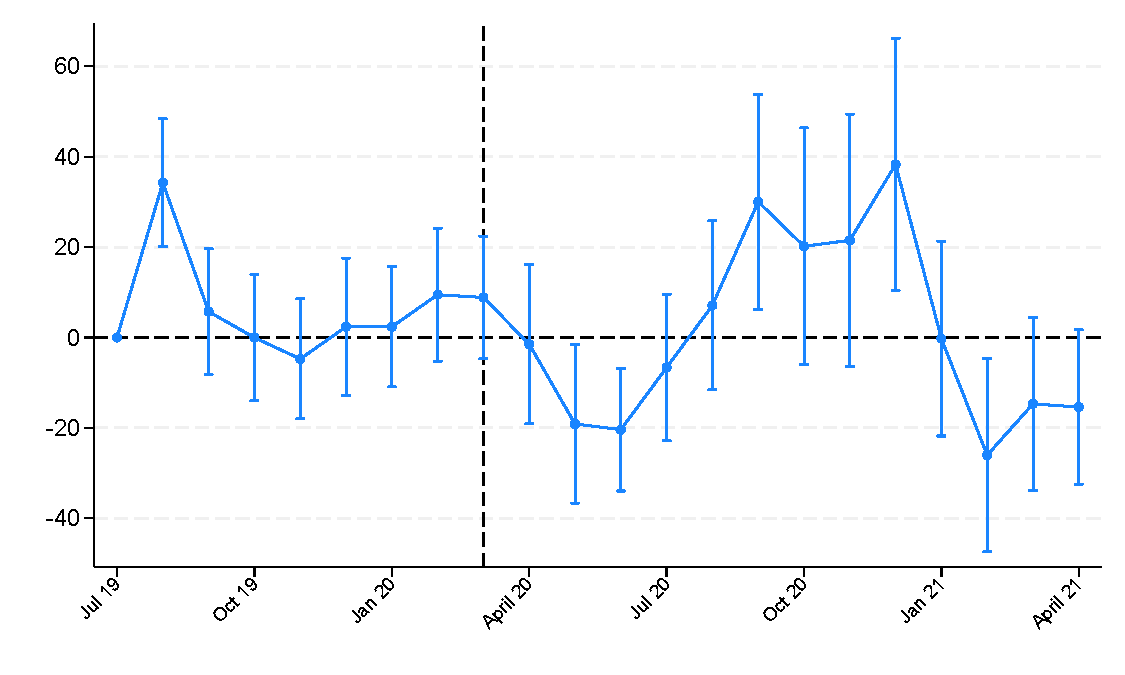
\includegraphics[width=0.998\textwidth]{../results/figures/did_loan_amount_exposure_march_dummy.pdf}
        \caption{ Loan amount }\label{fig:loan_amount}
       \end{subfigure}
       \begin{subfigure}[b]{0.49\textwidth}
        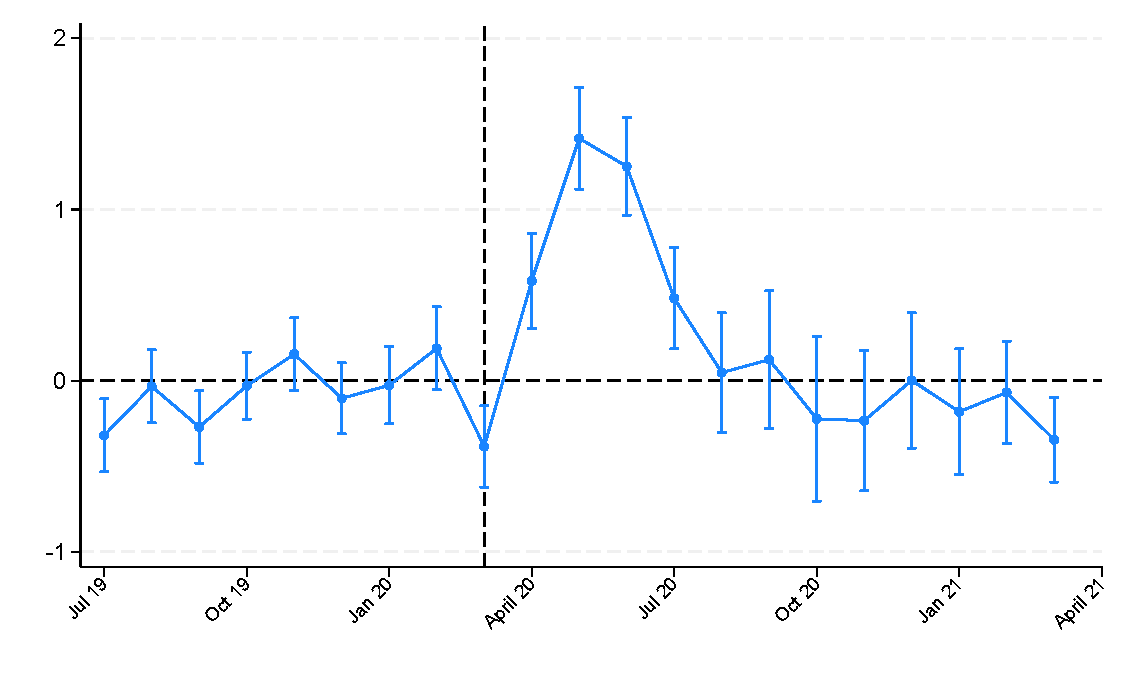
\includegraphics[width=0.998\textwidth]{../results/figures/did_winner_bid_exposure_march_dummy.pdf}
        \caption{ Winner bid }\label{fig:winner_bid}
       \end{subfigure}
       \caption{Effect of QE on Ob Auctions using exposure dummy on March 2020.}\label{fig:did_exp_amount}
     \begin{minipage}{\textwidth}
        \footnotesize{\textit{Notes:}  The figure coefficients of the regression above for loan amounts and winner bid. The vertical line is March 1.  Robust standard errors are used. }
        \end{minipage}
  \end{figure}
  

\begin{figure}[h]
    \centering
    \begin{subfigure}[b]{0.49\textwidth}
        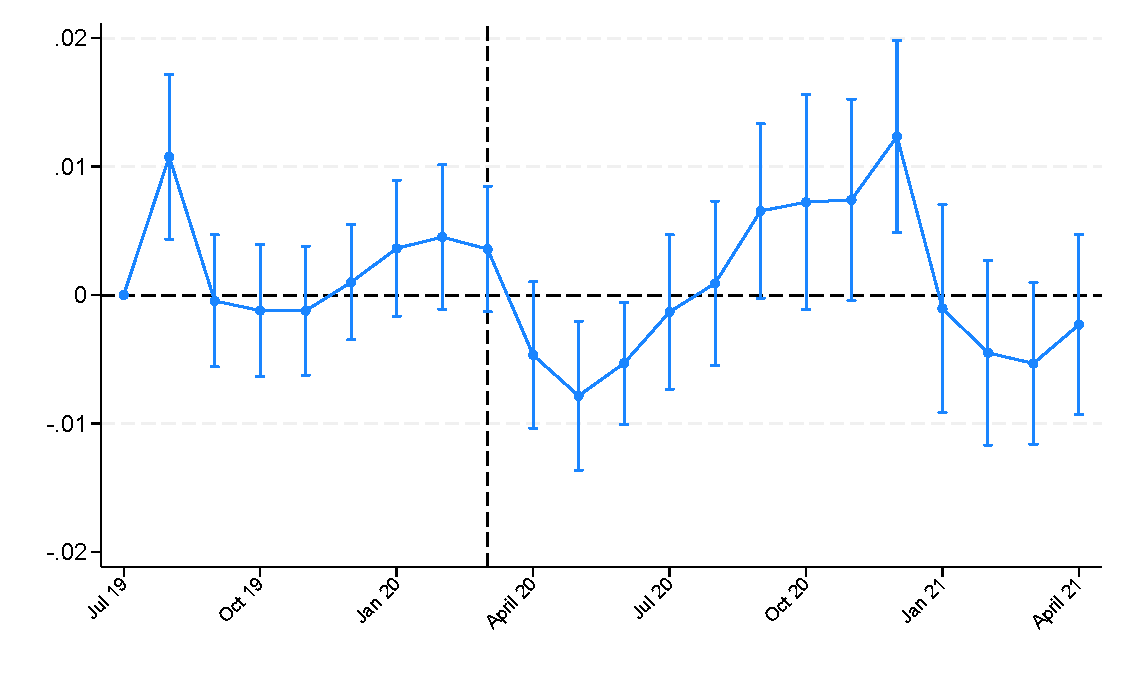
\includegraphics[width=0.998\textwidth]{../results/figures/did_loan_amount_expamount_march_dummy.pdf}
        \caption{ Loan amount }\label{fig:loan_amount}
       \end{subfigure}
       \begin{subfigure}[b]{0.49\textwidth}
        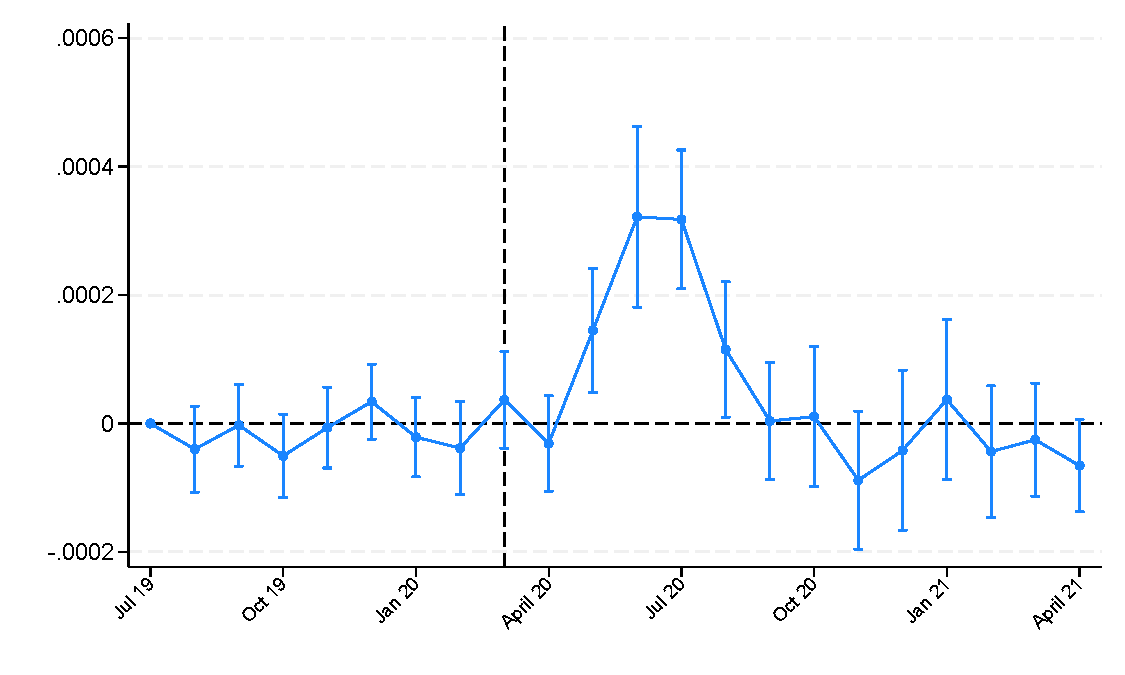
\includegraphics[width=0.998\textwidth]{../results/figures/did_winner_bid_expamount_march_dummy.pdf}
        \caption{ Winner bid }\label{fig:winner_bid}
       \end{subfigure}
       \caption{Effect of QE on Ob Auctions using exposure amount purchase on March 2020.}\label{fig:did_exp_amount}
     \begin{minipage}{\textwidth}
        \footnotesize{\textit{Notes:}  The figure coefficients of the regression above for loan amounts and winner bid. The vertical line is March 1.  Robust standard errors are used. }
        \end{minipage}
  \end{figure}
  


  \begin{figure}[h]
    \centering
    \begin{subfigure}[b]{0.49\textwidth}
        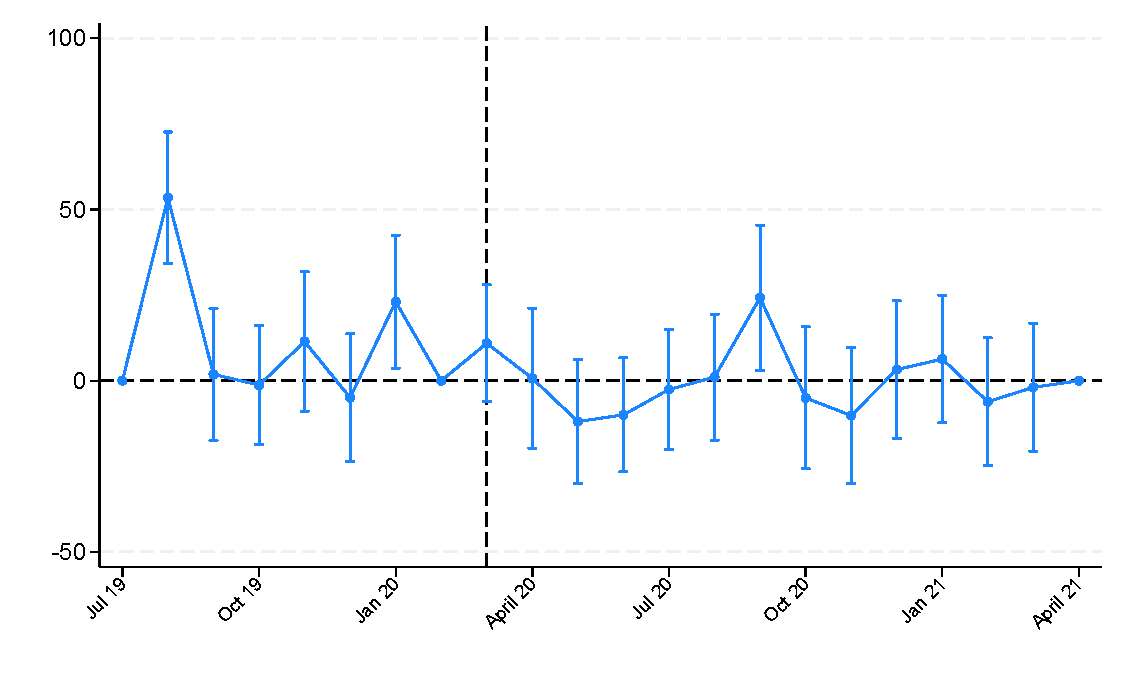
\includegraphics[width=0.998\textwidth]{../results/figures/did_loan_amount_exposure_dummy.pdf}
        \caption{ Loan amount }\label{fig:loan_amount}
       \end{subfigure}
       \begin{subfigure}[b]{0.49\textwidth}
        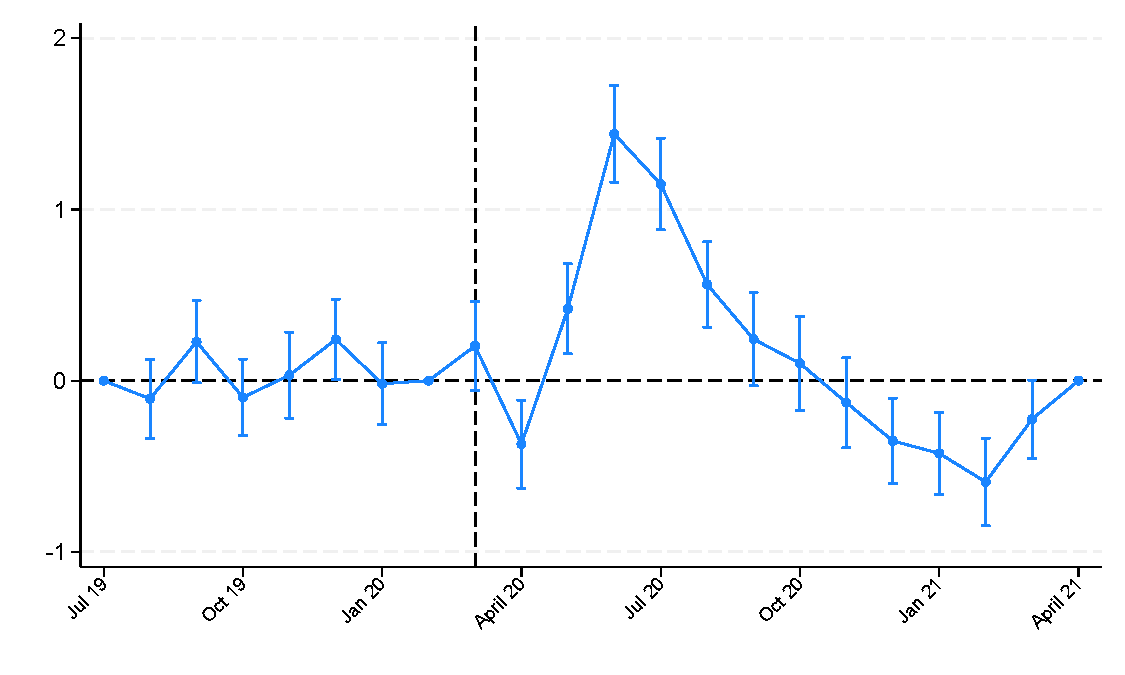
\includegraphics[width=0.998\textwidth]{../results/figures/did_winner_bid_exposure_dummy.pdf}
        \caption{ Winner bid }\label{fig:winner_bid}
       \end{subfigure}
       \caption{Robustness: Effect of QE on Ob Auctions using exposure dummy by month. }\label{fig:did_exp_amount}
     \begin{minipage}{\textwidth}
        \footnotesize{\textit{Notes:}  The figure coefficients of the regression above for loan amounts and winner bid. The vertical line is March 1.  Robust standard errors are used. }
        \end{minipage}
  \end{figure}
  

\begin{figure}[h]
    \centering
    \begin{subfigure}[b]{0.49\textwidth}
        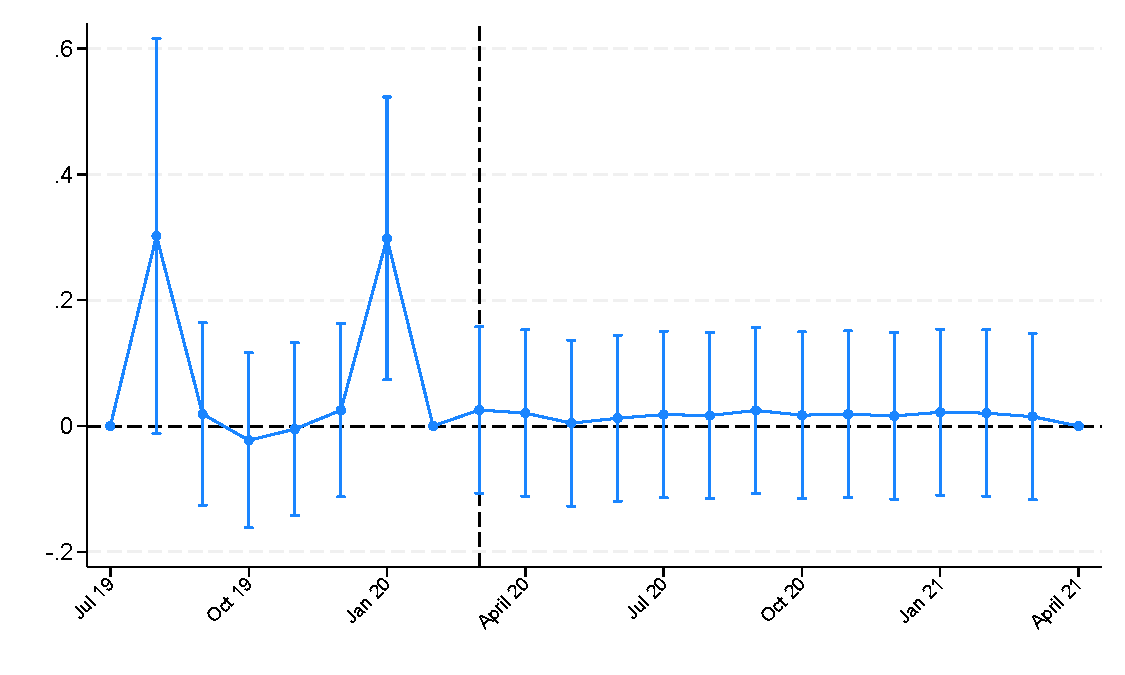
\includegraphics[width=0.998\textwidth]{../results/figures/did_loan_amount_expamount.pdf}
        \caption{ Loan amount }\label{fig:loan_amount}
       \end{subfigure}
       \begin{subfigure}[b]{0.49\textwidth}
        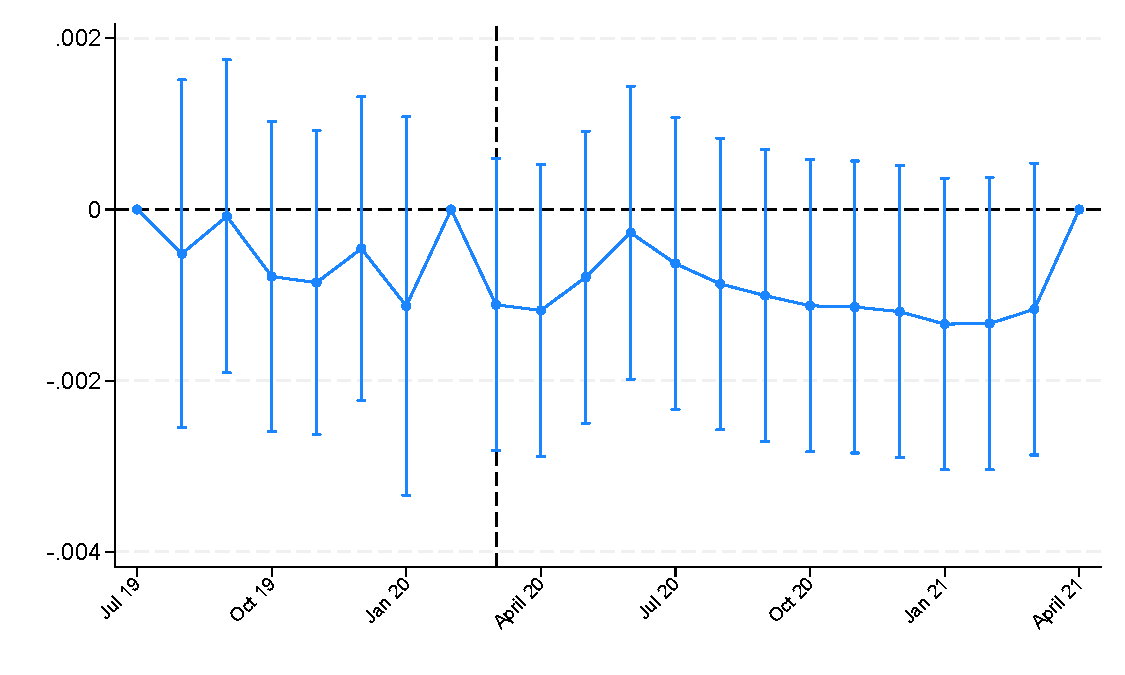
\includegraphics[width=0.998\textwidth]{../results/figures/did_winner_bid_expamount.pdf}
        \caption{ Winner bid }\label{fig:winner_bid}
       \end{subfigure}
       \caption{Robustness: Effect of QE on Ob Auctions using exposure amount purchase by month. }\label{fig:did_exp_amount}
     \begin{minipage}{\textwidth}
        \footnotesize{\textit{Notes:}  The figure coefficients of the regression above for loan amounts and winner bid. The vertical line is March 1.  Robust standard errors are used. }
        \end{minipage}
  \end{figure}
  

\end{document}
